

\tikzset{every picture/.style={line width=0.75pt}} %set default line width to 0.75pt

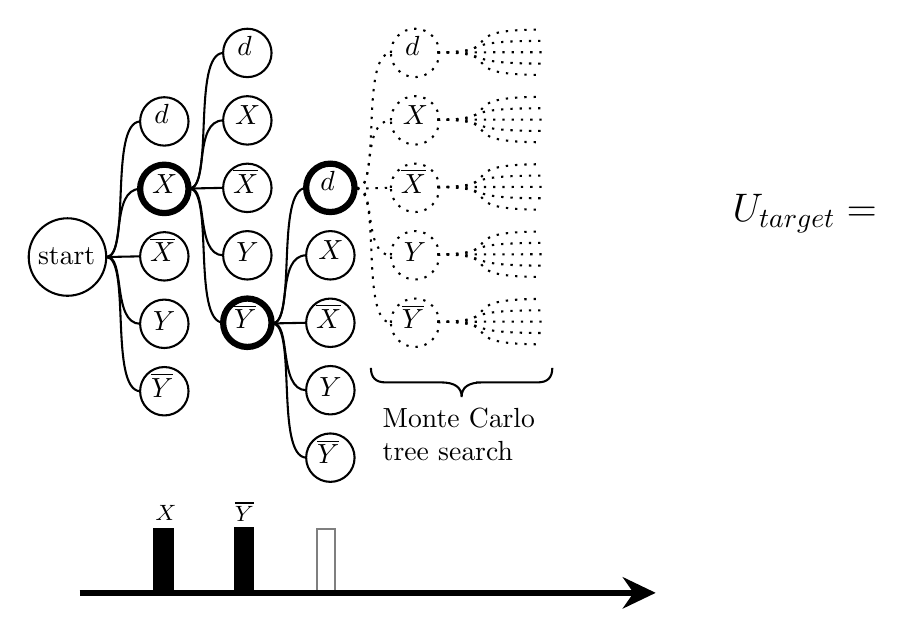
\begin{tikzpicture}[x=0.75pt,y=0.75pt,yscale=-1,xscale=1]
%uncomment if require: \path (0,300); %set diagram left start at 0, and has height of 300

%Shape: Circle [id:dp9046759261625568]
\draw   (77,60.67) .. controls (77,54.22) and (82.22,49) .. (88.67,49) .. controls (95.11,49) and (100.33,54.22) .. (100.33,60.67) .. controls (100.33,67.11) and (95.11,72.33) .. (88.67,72.33) .. controls (82.22,72.33) and (77,67.11) .. (77,60.67) -- cycle ;
%Shape: Circle [id:dp2720164009687023]
\draw  [line width=2.25]  (77,93.17) .. controls (77,86.73) and (82.22,81.5) .. (88.67,81.5) .. controls (95.11,81.5) and (100.33,86.73) .. (100.33,93.17) .. controls (100.33,99.61) and (95.11,104.84) .. (88.67,104.84) .. controls (82.22,104.84) and (77,99.61) .. (77,93.17) -- cycle ;
%Shape: Circle [id:dp7036273582393138]
\draw   (77,125.67) .. controls (77,119.23) and (82.22,114.01) .. (88.67,114.01) .. controls (95.11,114.01) and (100.33,119.23) .. (100.33,125.67) .. controls (100.33,132.12) and (95.11,137.34) .. (88.67,137.34) .. controls (82.22,137.34) and (77,132.12) .. (77,125.67) -- cycle ;
%Shape: Circle [id:dp30398985571820214]
\draw   (77,158.18) .. controls (77,151.73) and (82.22,146.51) .. (88.67,146.51) .. controls (95.11,146.51) and (100.33,151.73) .. (100.33,158.18) .. controls (100.33,164.62) and (95.11,169.84) .. (88.67,169.84) .. controls (82.22,169.84) and (77,164.62) .. (77,158.18) -- cycle ;
%Shape: Circle [id:dp47733742173317295]
\draw   (77,190.67) .. controls (77,184.22) and (82.22,179) .. (88.67,179) .. controls (95.11,179) and (100.33,184.22) .. (100.33,190.67) .. controls (100.33,197.11) and (95.11,202.33) .. (88.67,202.33) .. controls (82.22,202.33) and (77,197.11) .. (77,190.67) -- cycle ;
%Curve Lines [id:da15003157478518636]
\draw    (60.67,126) .. controls (72.67,126) and (62,61.33) .. (77,60.67) ;
%Curve Lines [id:da8250791502123043]
\draw    (60.67,126) .. controls (70,126) and (62.67,93.33) .. (77,93.17) ;
%Curve Lines [id:da9035503948679597]
\draw    (60.67,126) .. controls (72.67,126) and (62,189.97) .. (77,190.67) ;
%Curve Lines [id:da20495653155266225]
\draw    (60.67,126) .. controls (70,124.67) and (63.33,158) .. (77,158.18) ;
%Straight Lines [id:da5161405015219109]
\draw    (60.67,126) -- (77,125.67) ;

%Shape: Circle [id:dp6856566096163164]
\draw   (23.33,126) .. controls (23.33,115.69) and (31.69,107.33) .. (42,107.33) .. controls (52.31,107.33) and (60.67,115.69) .. (60.67,126) .. controls (60.67,136.31) and (52.31,144.67) .. (42,144.67) .. controls (31.69,144.67) and (23.33,136.31) .. (23.33,126) -- cycle ;
%Shape: Circle [id:dp3943399377951582]
\draw   (117,27.67) .. controls (117,21.22) and (122.22,16) .. (128.67,16) .. controls (135.11,16) and (140.33,21.22) .. (140.33,27.67) .. controls (140.33,34.11) and (135.11,39.33) .. (128.67,39.33) .. controls (122.22,39.33) and (117,34.11) .. (117,27.67) -- cycle ;
%Shape: Circle [id:dp027403378825546554]
\draw   (117,60.17) .. controls (117,53.73) and (122.22,48.5) .. (128.67,48.5) .. controls (135.11,48.5) and (140.33,53.73) .. (140.33,60.17) .. controls (140.33,66.61) and (135.11,71.84) .. (128.67,71.84) .. controls (122.22,71.84) and (117,66.61) .. (117,60.17) -- cycle ;
%Shape: Circle [id:dp18742338383587276]
\draw   (117,92.67) .. controls (117,86.23) and (122.22,81.01) .. (128.67,81.01) .. controls (135.11,81.01) and (140.33,86.23) .. (140.33,92.67) .. controls (140.33,99.12) and (135.11,104.34) .. (128.67,104.34) .. controls (122.22,104.34) and (117,99.12) .. (117,92.67) -- cycle ;
%Shape: Circle [id:dp9772441176859072]
\draw   (117,125.18) .. controls (117,118.73) and (122.22,113.51) .. (128.67,113.51) .. controls (135.11,113.51) and (140.33,118.73) .. (140.33,125.18) .. controls (140.33,131.62) and (135.11,136.84) .. (128.67,136.84) .. controls (122.22,136.84) and (117,131.62) .. (117,125.18) -- cycle ;
%Shape: Circle [id:dp6375454025693941]
\draw  [line width=2.25]  (117,157.67) .. controls (117,151.22) and (122.22,146) .. (128.67,146) .. controls (135.11,146) and (140.33,151.22) .. (140.33,157.67) .. controls (140.33,164.11) and (135.11,169.33) .. (128.67,169.33) .. controls (122.22,169.33) and (117,164.11) .. (117,157.67) -- cycle ;
%Curve Lines [id:da7935513938946654]
\draw    (100.67,93) .. controls (112.67,93) and (102,28.33) .. (117,27.67) ;
%Curve Lines [id:da9090746048189753]
\draw    (100.67,93) .. controls (110,93) and (102.67,60.33) .. (117,60.17) ;
%Curve Lines [id:da08019414129507907]
\draw    (100.67,93) .. controls (112.67,93) and (102,156.97) .. (117,157.67) ;
%Curve Lines [id:da8818934103423806]
\draw    (100.67,93) .. controls (110,91.67) and (103.33,125) .. (117,125.18) ;
%Straight Lines [id:da3600527836975942]
\draw    (100.67,93) -- (117,92.67) ;

%Shape: Circle [id:dp37197107969313614]
\draw  [line width=2.25]  (157,92.67) .. controls (157,86.22) and (162.22,81) .. (168.67,81) .. controls (175.11,81) and (180.33,86.22) .. (180.33,92.67) .. controls (180.33,99.11) and (175.11,104.33) .. (168.67,104.33) .. controls (162.22,104.33) and (157,99.11) .. (157,92.67) -- cycle ;
%Shape: Circle [id:dp6275475319115866]
\draw   (157,125.17) .. controls (157,118.73) and (162.22,113.5) .. (168.67,113.5) .. controls (175.11,113.5) and (180.33,118.73) .. (180.33,125.17) .. controls (180.33,131.61) and (175.11,136.84) .. (168.67,136.84) .. controls (162.22,136.84) and (157,131.61) .. (157,125.17) -- cycle ;
%Shape: Circle [id:dp20634171892967257]
\draw   (157,157.67) .. controls (157,151.23) and (162.22,146.01) .. (168.67,146.01) .. controls (175.11,146.01) and (180.33,151.23) .. (180.33,157.67) .. controls (180.33,164.12) and (175.11,169.34) .. (168.67,169.34) .. controls (162.22,169.34) and (157,164.12) .. (157,157.67) -- cycle ;
%Shape: Circle [id:dp005375931541727663]
\draw   (157,190.18) .. controls (157,183.73) and (162.22,178.51) .. (168.67,178.51) .. controls (175.11,178.51) and (180.33,183.73) .. (180.33,190.18) .. controls (180.33,196.62) and (175.11,201.84) .. (168.67,201.84) .. controls (162.22,201.84) and (157,196.62) .. (157,190.18) -- cycle ;
%Shape: Circle [id:dp30698472035152635]
\draw   (157,222.67) .. controls (157,216.22) and (162.22,211) .. (168.67,211) .. controls (175.11,211) and (180.33,216.22) .. (180.33,222.67) .. controls (180.33,229.11) and (175.11,234.33) .. (168.67,234.33) .. controls (162.22,234.33) and (157,229.11) .. (157,222.67) -- cycle ;
%Curve Lines [id:da24565594693868897]
\draw    (140.67,158) .. controls (152.67,158) and (142,93.33) .. (157,92.67) ;
%Curve Lines [id:da5338540044019582]
\draw    (140.67,158) .. controls (150,158) and (142.67,125.33) .. (157,125.17) ;
%Curve Lines [id:da9225241366716022]
\draw    (140.67,158) .. controls (152.67,158) and (142,221.97) .. (157,222.67) ;
%Curve Lines [id:da15552356993518202]
\draw    (140.67,158) .. controls (150,156.67) and (143.33,190) .. (157,190.18) ;
%Straight Lines [id:da21353471154132975]
\draw    (140.67,158) -- (157,157.67) ;

%Shape: Circle [id:dp04181875688613368]
\draw  [dash pattern={on 0.84pt off 2.51pt}][line width=0.75]  (197.8,27.67) .. controls (197.8,21.22) and (203.02,16) .. (209.47,16) .. controls (215.91,16) and (221.13,21.22) .. (221.13,27.67) .. controls (221.13,34.11) and (215.91,39.33) .. (209.47,39.33) .. controls (203.02,39.33) and (197.8,34.11) .. (197.8,27.67) -- cycle ;
%Shape: Circle [id:dp9520151357098714]
\draw  [dash pattern={on 0.84pt off 2.51pt}] (197.8,60.17) .. controls (197.8,53.73) and (203.02,48.5) .. (209.47,48.5) .. controls (215.91,48.5) and (221.13,53.73) .. (221.13,60.17) .. controls (221.13,66.61) and (215.91,71.84) .. (209.47,71.84) .. controls (203.02,71.84) and (197.8,66.61) .. (197.8,60.17) -- cycle ;
%Shape: Circle [id:dp6091644032597949]
\draw  [dash pattern={on 0.84pt off 2.51pt}] (197.8,92.67) .. controls (197.8,86.23) and (203.02,81.01) .. (209.47,81.01) .. controls (215.91,81.01) and (221.13,86.23) .. (221.13,92.67) .. controls (221.13,99.12) and (215.91,104.34) .. (209.47,104.34) .. controls (203.02,104.34) and (197.8,99.12) .. (197.8,92.67) -- cycle ;
%Shape: Circle [id:dp30106591129563065]
\draw  [dash pattern={on 0.84pt off 2.51pt}] (197.8,125.18) .. controls (197.8,118.73) and (203.02,113.51) .. (209.47,113.51) .. controls (215.91,113.51) and (221.13,118.73) .. (221.13,125.18) .. controls (221.13,131.62) and (215.91,136.84) .. (209.47,136.84) .. controls (203.02,136.84) and (197.8,131.62) .. (197.8,125.18) -- cycle ;
%Shape: Circle [id:dp11491575042636026]
\draw  [dash pattern={on 0.84pt off 2.51pt}] (197.8,157.67) .. controls (197.8,151.22) and (203.02,146) .. (209.47,146) .. controls (215.91,146) and (221.13,151.22) .. (221.13,157.67) .. controls (221.13,164.11) and (215.91,169.33) .. (209.47,169.33) .. controls (203.02,169.33) and (197.8,164.11) .. (197.8,157.67) -- cycle ;
%Curve Lines [id:da6833103888584182]
\draw  [dash pattern={on 0.84pt off 2.51pt}]  (181.47,93) .. controls (193.47,93) and (182.8,28.33) .. (197.8,27.67) ;
%Curve Lines [id:da7170577068303761]
\draw  [dash pattern={on 0.84pt off 2.51pt}]  (181.47,93) .. controls (190.8,93) and (183.47,60.33) .. (197.8,60.17) ;
%Curve Lines [id:da9592178971273932]
\draw  [dash pattern={on 0.84pt off 2.51pt}]  (181.47,93) .. controls (193.47,93) and (182.8,156.97) .. (197.8,157.67) ;
%Curve Lines [id:da8897306480704943]
\draw  [dash pattern={on 0.84pt off 2.51pt}]  (181.47,93) .. controls (190.8,91.67) and (184.13,125) .. (197.8,125.18) ;
%Straight Lines [id:da5951582855021698]
\draw  [dash pattern={on 0.84pt off 2.51pt}]  (181.47,93) -- (197.8,92.67) ;
%Curve Lines [id:da8597674854104052]
\draw  [dash pattern={on 0.84pt off 2.51pt}]  (220.27,157.19) .. controls (257.1,157.19) and (224.36,146.31) .. (270.4,146.2) ;
%Curve Lines [id:da6456542749429195]
\draw  [dash pattern={on 0.84pt off 2.51pt}]  (220.27,157.19) .. controls (248.91,157.19) and (226.41,151.69) .. (270.4,151.67) ;
%Curve Lines [id:da20333203775585673]
\draw  [dash pattern={on 0.84pt off 2.51pt}]  (220.27,157.19) .. controls (257.1,157.19) and (224.36,167.95) .. (270.4,168.07) ;
%Curve Lines [id:da9570130583498357]
\draw  [dash pattern={on 0.84pt off 2.51pt}]  (220.27,157.19) .. controls (248.91,156.97) and (228.45,162.57) .. (270.4,162.6) ;
%Straight Lines [id:da7018938601767097]
\draw  [dash pattern={on 0.84pt off 2.51pt}]  (220.27,157.19) -- (270.4,157.13) ;

%Shape: Brace [id:dp7050804983181456]
\draw   (188.2,179.4) .. controls (188.2,184.07) and (190.53,186.4) .. (195.2,186.4) -- (221.9,186.4) .. controls (228.57,186.4) and (231.9,188.73) .. (231.9,193.4) .. controls (231.9,188.73) and (235.23,186.4) .. (241.9,186.4)(238.9,186.4) -- (268.6,186.4) .. controls (273.27,186.4) and (275.6,184.07) .. (275.6,179.4) ;
%Curve Lines [id:da5250288933388279]
\draw  [dash pattern={on 0.84pt off 2.51pt}]  (220.27,124.73) .. controls (257.1,124.73) and (224.36,113.85) .. (270.4,113.74) ;
%Curve Lines [id:da6691887839152604]
\draw  [dash pattern={on 0.84pt off 2.51pt}]  (220.27,124.73) .. controls (248.91,124.73) and (226.41,119.23) .. (270.4,119.21) ;
%Curve Lines [id:da5764348202911984]
\draw  [dash pattern={on 0.84pt off 2.51pt}]  (220.27,124.73) .. controls (257.1,124.73) and (224.36,135.49) .. (270.4,135.61) ;
%Curve Lines [id:da03866317180478207]
\draw  [dash pattern={on 0.84pt off 2.51pt}]  (220.27,124.73) .. controls (248.91,124.51) and (228.45,130.11) .. (270.4,130.14) ;
%Straight Lines [id:da948997784648149]
\draw  [dash pattern={on 0.84pt off 2.51pt}]  (220.27,124.73) -- (270.4,124.67) ;

%Curve Lines [id:da8933530934097043]
\draw  [dash pattern={on 0.84pt off 2.51pt}]  (220.27,92.28) .. controls (257.1,92.28) and (224.36,81.41) .. (270.4,81.29) ;
%Curve Lines [id:da6635023036458383]
\draw  [dash pattern={on 0.84pt off 2.51pt}]  (220.27,92.28) .. controls (248.91,92.28) and (226.41,86.79) .. (270.4,86.76) ;
%Curve Lines [id:da9007691742812654]
\draw  [dash pattern={on 0.84pt off 2.51pt}]  (220.27,92.28) .. controls (257.1,92.28) and (224.36,103.04) .. (270.4,103.16) ;
%Curve Lines [id:da24220817594865474]
\draw  [dash pattern={on 0.84pt off 2.51pt}]  (220.27,92.28) .. controls (248.91,92.06) and (228.45,97.67) .. (270.4,97.7) ;
%Straight Lines [id:da025844200521988325]
\draw  [dash pattern={on 0.84pt off 2.51pt}]  (220.27,92.28) -- (270.4,92.23) ;

%Curve Lines [id:da7376226380396587]
\draw  [dash pattern={on 0.84pt off 2.51pt}]  (220.27,59.84) .. controls (257.1,59.84) and (224.36,48.96) .. (270.4,48.85) ;
%Curve Lines [id:da8154456306200297]
\draw  [dash pattern={on 0.84pt off 2.51pt}]  (220.27,59.84) .. controls (248.91,59.84) and (226.41,54.34) .. (270.4,54.31) ;
%Curve Lines [id:da16175976651173296]
\draw  [dash pattern={on 0.84pt off 2.51pt}]  (220.27,59.84) .. controls (257.1,59.84) and (224.36,70.6) .. (270.4,70.71) ;
%Curve Lines [id:da9797301308280535]
\draw  [dash pattern={on 0.84pt off 2.51pt}]  (220.27,59.84) .. controls (248.91,59.61) and (228.45,65.22) .. (270.4,65.25) ;
%Straight Lines [id:da528793851368276]
\draw  [dash pattern={on 0.84pt off 2.51pt}]  (220.27,59.84) -- (270.4,59.78) ;

%Curve Lines [id:da32601222649721584]
\draw  [dash pattern={on 0.84pt off 2.51pt}]  (220.27,27.39) .. controls (257.1,27.39) and (224.36,16.51) .. (270.4,16.4) ;
%Curve Lines [id:da3229850987139369]
\draw  [dash pattern={on 0.84pt off 2.51pt}]  (220.27,27.39) .. controls (248.91,27.39) and (226.41,21.89) .. (270.4,21.87) ;
%Curve Lines [id:da856781680693991]
\draw  [dash pattern={on 0.84pt off 2.51pt}]  (220.27,27.39) .. controls (257.1,27.39) and (224.36,38.15) .. (270.4,38.27) ;
%Curve Lines [id:da950898346766704]
\draw  [dash pattern={on 0.84pt off 2.51pt}]  (220.27,27.39) .. controls (248.91,27.17) and (228.45,32.77) .. (270.4,32.8) ;
%Straight Lines [id:da5870679311667073]
\draw  [dash pattern={on 0.84pt off 2.51pt}]  (220.27,27.39) -- (270.4,27.33) ;

%Straight Lines [id:da037704353344952146]
\draw [line width=2.25]    (47.8,287.8) -- (320.4,287.8) ;
\draw [shift={(325.4,287.8)}, rotate = 180] [fill={rgb, 255:red, 0; green, 0; blue, 0 }  ][line width=0.08]  [draw opacity=0] (16.07,-7.72) -- (0,0) -- (16.07,7.72) -- (10.67,0) -- cycle    ;
%Shape: Rectangle [id:dp002389671521099812]
\draw  [fill={rgb, 255:red, 0; green, 0; blue, 0 }  ,fill opacity=1 ] (83.8,257) -- (92.6,257) -- (92.6,286.8) -- (83.8,286.8) -- cycle ;
%Shape: Rectangle [id:dp3916809463858497]
\draw  [fill={rgb, 255:red, 0; green, 0; blue, 0 }  ,fill opacity=1 ] (122.6,256.6) -- (131.4,256.6) -- (131.4,286.4) -- (122.6,286.4) -- cycle ;
%Shape: Rectangle [id:dp617205458629722]
\draw  [color={rgb, 255:red, 0; green, 0; blue, 0 }  ,draw opacity=0.5 ] (162.2,257.2) -- (171,257.2) -- (171,287) -- (162.2,287) -- cycle ;

% Text Node
\draw (41.59,125.5) node   [align=left] {start};
% Text Node
\draw (122.33,18.07) node [anchor=north west][inner sep=0.75pt]    {$d$};
% Text Node
\draw (120.83,147.4) node [anchor=north west][inner sep=0.75pt]    {$\overline{Y}$};
% Text Node
\draw (121.83,117.73) node [anchor=north west][inner sep=0.75pt]    {$Y$};
% Text Node
\draw (120.33,82.07) node [anchor=north west][inner sep=0.75pt]    {$\overline{X}$};
% Text Node
\draw (121.33,51.73) node [anchor=north west][inner sep=0.75pt]    {$X$};
% Text Node
\draw (81.33,84.73) node [anchor=north west][inner sep=0.75pt]    {$X$};
% Text Node
\draw (80.33,115.07) node [anchor=north west][inner sep=0.75pt]    {$\overline{X}$};
% Text Node
\draw (81.83,150.73) node [anchor=north west][inner sep=0.75pt]    {$Y$};
% Text Node
\draw (80.83,180.4) node [anchor=north west][inner sep=0.75pt]    {$\overline{Y}$};
% Text Node
\draw (82.33,51.07) node [anchor=north west][inner sep=0.75pt]    {$d$};
% Text Node
\draw (162.33,83.07) node [anchor=north west][inner sep=0.75pt]    {$d$};
% Text Node
\draw (160.83,212.4) node [anchor=north west][inner sep=0.75pt]    {$\overline{Y}$};
% Text Node
\draw (161.83,182.73) node [anchor=north west][inner sep=0.75pt]    {$Y$};
% Text Node
\draw (160.33,147.07) node [anchor=north west][inner sep=0.75pt]    {$\overline{X}$};
% Text Node
\draw (161.33,116.73) node [anchor=north west][inner sep=0.75pt]    {$X$};
% Text Node
\draw (202.13,51.73) node [anchor=north west][inner sep=0.75pt]    {$X$};
% Text Node
\draw (201.13,82.07) node [anchor=north west][inner sep=0.75pt]    {$\overline{X}$};
% Text Node
\draw (202.63,117.73) node [anchor=north west][inner sep=0.75pt]    {$Y$};
% Text Node
\draw (201.63,147.4) node [anchor=north west][inner sep=0.75pt]    {$\overline{Y}$};
% Text Node
\draw (203.13,18.07) node [anchor=north west][inner sep=0.75pt]    {$d$};
% Text Node
\draw (192.4,197.4) node [anchor=north west][inner sep=0.75pt]   [align=left] {Monte Carlo\\tree search};
% Text Node
\draw (82.8,244) node [anchor=north west][inner sep=0.75pt]  [font=\footnotesize]  {$X$};
% Text Node
\draw (121.2,242.2) node [anchor=north west][inner sep=0.75pt]  [font=\footnotesize]  {$\overline{Y}$};
% Text Node
\draw (313.43,93) node  [font=\Huge]  {$\dotsc $};
% Text Node
\draw (361,94.4) node [anchor=north west][inner sep=0.75pt]  [font=\Large]  {$U_{\text{target}} = \identity$};


\end{tikzpicture}
